\documentclass{article}


\usepackage[margin=1in]{geometry}
\usepackage{amsmath}
\usepackage{graphicx}
\usepackage{tabu}
\usepackage{float}
\usepackage{listings}
\usepackage{color}


\author{Zachary Vogel\quad Chuyi Liu}
\title{Real Time Embedded Exercise 1\\ ECEN 5623}
\date{\today}

\begin{document}





\maketitle


\section*{Problem 1}
Here one can see the timing diagram for the three services. Since, service one is requested every 3 milliseconds, it has the highest priority. The overall Utilization of this system is $U=\frac{14}{15}=93.3\%$. I believe the schedule is feasible because the context and task switching for 3 services should reasonably be under 6\%. This is the case despite the system failing the least upper bound defined by rate monotonic analysis. I would say that the utillization is probably higher than desired
and it wouldn't be surprising if it missed a deadline in the real world. Theoretically, it never would, but if a task took even slightly longer than the expected time the system could fail.
\begin{figure}[H]
    \centering
    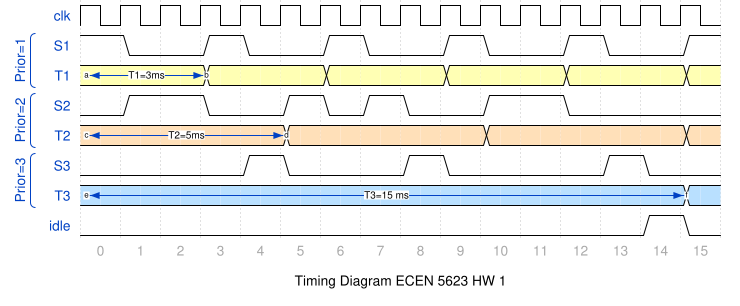
\includegraphics[width=0.9\textwidth]{HW1_TIME.png}
\end{figure}

\section*{Problem 2}
\subsection*{Summarizing the Document}
The author, Peter Adler, begins by discussing his background and his work for the lab. Then he goes into some of the constraints that they had to deal with. Namely that they didn't have much erasable memory, and had upwards of 7 programs using the same addresses. This forced them to do extensive testing to make sure programs weren't using the same memory cells at the same time. He also notes that most of the programs ran from their 36,864 15 bit words of fixed memory. The exception to this
was the Apollo 14 incident.\\
His coworker, Don Eyles, had figured out how to patch a program with a faulty abort switch. This patch had to be entered manually by the crew. The author also notes the achievement of developing a real-time multi-tasking, interrupt driven time-dependent, operating system in 1967. A lot of programs required the same data values, these were stored in shared memory. Each job was also allocated 12 erasable memory locations, and given 44 more erasable words, known as a VAC, if they were needed. When a job was
scheduled, if it needed VAC memory, the OS searched the five VAC areas to determine if one was available. If it wasn't the program would branch to the Alarm/abort routine and set Alarm 1201. Similarly, if none of the core sets were available it would set Alarm 1202.\\
What happened with Apollo 11, was that the memory was filled up and a 1202 alarm was generated. Then a 1201 occurred because of this. The fill up happened because of a misconfiguration of radar switches. After that, the computer reset itself, and tried to start programs near the execution point where they failed. Basically, every time a 1201 or 1202 occurred, the computer rebooted, restarted the important jobs, but did not restart all the radar jobs that originally caused the 1201/1202. Due to extensive testing, the people who designed the system knew
this wouldn't cause a full failure.

\subsection*{Root cause of the Overload? Violation of RMS?}
The root cause of the overload was a misconfiguration of the radar switches that caused too many tasks to be created. Most of these were unnecessary. It violated rate-monotonic scheduling by sharing memory, and not having preemption. Basically, a bunch of the same unimportant tasks were running, but did not get preempted.

\subsection*{RM LUB Plot}
Basically, Rate monotonic scheduling guarantees one can have at least 70\% CPU utilization for any amount of tasks. As more and more tasks are implemented, the bound gets closer and closer to 70\%. This is evident below in the graph where CPU utilization is on the y axis, and number of processes is on the x axis. The margin for RM analysis caps out at 30\%. 3 assumptions that RM analysis makes are that, all tasks have periodic requests with constant interval between request, that the
run-time of each task is constant, and that each task should finish completion before the next occurs. The last one is why Apollo 11 breaks RM policy.
\begin{figure}[H]
    \centering
    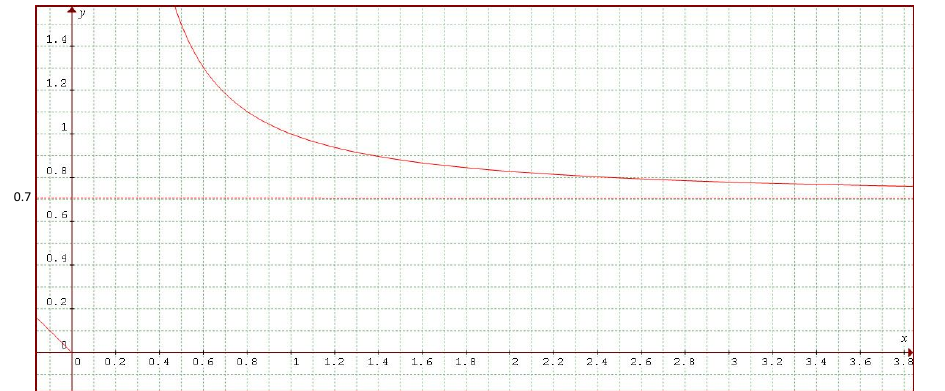
\includegraphics[width=0.9\textwidth]{HW1_P2.png}
\end{figure}
As for things I don't understand. I'm unsure how they determined the restrictions on the analysis that they did. I also wonder if you could do a least common multiple divided by 2 type analysis for the system. Most of the time I think one could get away with that because it could be extended relatively easily with a few simple calculations. I'm really not clear on how the LCM analysis works when the LCM is really large. They don't really plot a system timing diagram when the LCM is
100s of times the clock speed do they?


\subsection*{Would RM analysis have worked?}
RM analysis would not have even applied to the Apollo 11 program because one of the fundamental assumptions is broken in their system. The radar service task is created multiple times before each individual task is finished. Also, RM analysis gives highest priority to the most frequent task, which in this case might have been the radar service. If they guaranteed that the radar task did not get called multiple times, and that other tasks had higher frequency and therefore priority, RM analysis
would have probably worked.

\section*{Problem 3}
\subsection*{Proof our code ran}
\begin{figure}[H]
    \centering
    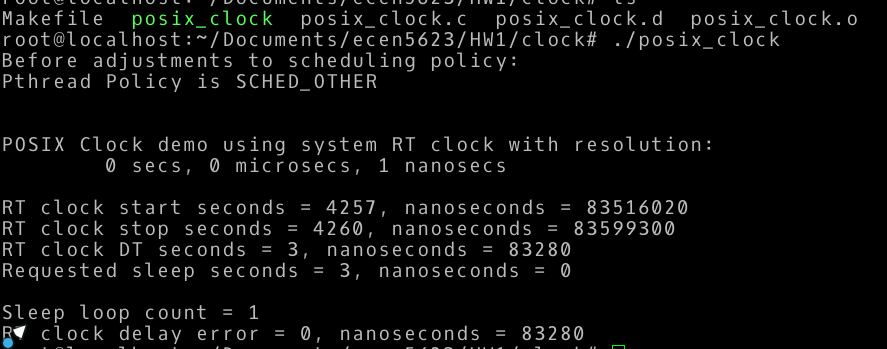
\includegraphics[width=0.8\textwidth]{HW1_P3_code.png}
\end{figure}

\subsection*{Description of Code}
The program posix\_clock is trying to demonstrate the usage of the time library to measure time execution. It uses one thread and the clock\_gettime function to determine how long a delay lasts. Before the delay it takes the time and after the delay it takes the time. Then it finds the difference to determine how long the delay lasted based on the CLOCK\_REALTIME. If this time is equivalent to the amount of time that where the system slept using the commnad nanosleep, then everything
is accurate. In our example, the difference between the requested delay and the actual computation was 83,280 nanoseconds over a 3 second period. One could do further analysis by changing the requested delay, and seeing how that difference scaled.
This program also did an interesting thing with the thread. It set the scheduler attributes to be the linux fifo scheduler, and set the priority to the maximum priority possible for the system. This ensured that this process had priority over everything else, which made the calculations more accurate.

\subsection*{Why are each of these things important?}

\indent Low interrupt handler latency is important because it implies that the interrupt handler has relatively low CPU utilization compared to a handler with a higher latency. In other words, a system with low interrupt handler latency spends less time dealing with interrupts and more time actually running the system's services. Also, low interrupt handler latency means.\\

Low context switch time is also essential to a good embedded operating system. In systems with many processes that are switching, the system can't afford to be slowed down by storing the states of all of the processes when switching between them. Preemption and task switching is great, but not if the system spends more time storing the context of each task rather than running real code. Combined with a low interrupt handler latency, this will allow a system to spend as much time as possible on
executing the actual services in the system. Basically, both of these come down to spending the most amount of time possible on the actual tasks.\\

Stable timer interrupts are one of the most essential things in real-time systems. If a system can't keep track of time accurately, how can it meet the deadlines it needs to meet. A schedule is only accurate if it is built on an accurate timing system. Without an accurate timer that doesn't change over time one can't guarantee that their processor will be interrupted on time.\\

\subsection*{RT-Clock Code Accuracy}
We don't believe the accuracy of the real time clock is perfect. This is because the fastest clock on the Altera DE1 board is only at 800MHz, and therefore couldn't keep track of nanoseconds. Even beyond that, the clock cycles have drift meaning they will have some error and won't be exactly 1/800Mhz in time. It is probably fairly accurate for microsecond type timing because than the drift and clock speed that isn't convenient could be accounted for.

\section*{Problem 4}
\subsection*{Proof Code Ran}
Proof simple-thread code ran:
\begin{figure}[H]
    \centering
    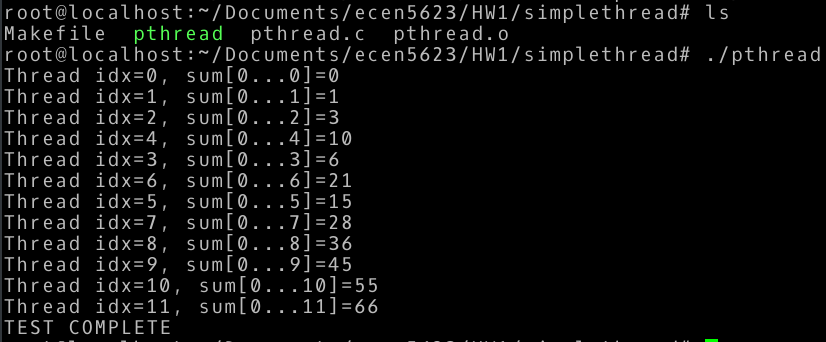
\includegraphics[width=0.8\textwidth]{HW1_P4_1.png}
\end{figure}
Proof example-sync code ran:
\begin{figure}[H]
    \centering
    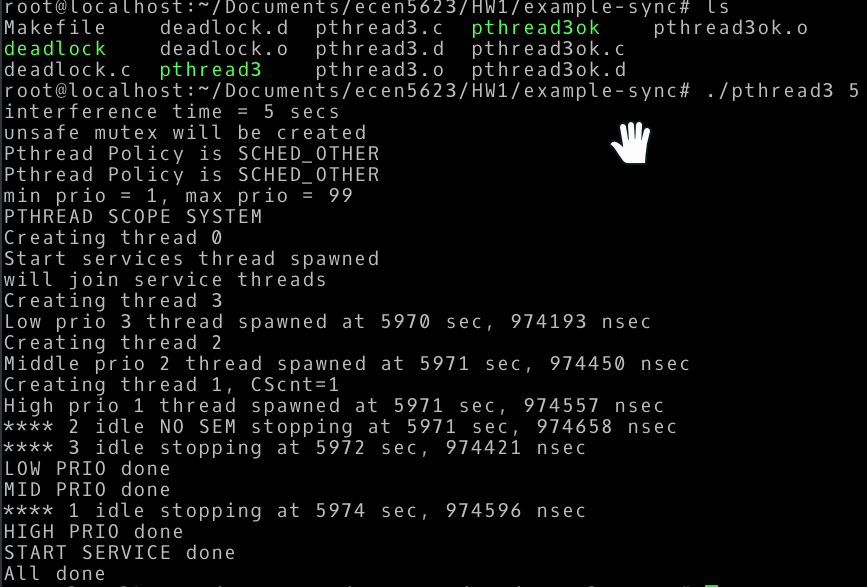
\includegraphics[width=0.8\textwidth]{HW1_P4_2.png}
\end{figure}
\subsection*{Description of Code}
The code in the simplethread folder is doing a relatively simple operation. It is doing a $\sum_{i=0}^{n-1}i$ where n is the number of threads. It is accomplishing this by making a global struct array that keeps the ID number of the threads (0 to 11). Then in a for loop it creates a thread using pthread\_create and passes in the thread Id number. That thread ID number is used in another for loop to bound the number of iterations. So you keep adding 1 to an iterator and summing that iterator
with the previous sum. The program waits for the threads to finish with another for loop and the function pthread\_join, which forces the CPU to wait until a thread is done before moving beyond that command. It also prints out all of the summed values in each thread. This system does not guarantee that each thread is summed in order of creation, which is why we don't see the printed values in size order.\\

The code in the example-sync folder spawned 4 threads. These were a start service, a high priority service, a mid priority service, and a low priority service. These services were setup to use the SCHED\_OTHER linux scheduler. The start service thread is run to generate the other 3 threads. It records what times these were launched and then waits for them to complete before exiting itself. The low and high priority threads run an idle task that uses a mutex to protect a critical section. This
critical section calculates fibonnaci sequences. Interestingly, the medium priority service does not use a mutex to protect it's calculations, but also does the fibonnaci calculations.

\subsection*{Description of VXworks Code and Implementation}
The VXworks code achieves the RM policy for the two fibonnaci calculation tasks using semaphores. The basic idea is that you start with 3 tasks. The first task is used to spawn the second and third. The second task has higher priority than the third, and the first has the highest of all. Thus, the first task starts, spawns the other two, and uses the semGive command to allow both of them to run. Then, it does a task delay for 20 seconds, which allows the two created tasks to run.
During that time, task 2, the 10 millisecond fibonnaci, will run and then hit the semTake(semF10,WAITFOREVER) command. This causes it to stop running and frees the CPU for other tasks to use. Then task 3, the 20 millisecond fibonnaci, runs for 10 milliseconds, but then the delay ends and the first task takes back over.\\

At that point, the first task uses semGive(semF10) to tell task 2 to run again. Then it waits another 20 milliseconds, task 2 runs for 10 milliseconds, hits semTake, and task 3 gets the CPU. This time, task 3 completes and runs semTake(semF20,WAITFOREVER). At this point, task 1 takes back over, gives semF10 again, and waits 10 more milliseconds. Task 2 runs again and then task 1 takes back over to give semF20 again along with another 10 millisecond delay. Task 3 runs for 10 milliseconds.
Task 1 then takes back over, and gives semF10 before waiting for 20 milliseconds again. This process in general repeats to get the timing diagram shown in the lab writeup.\\

Based on the grade rubric, we felt that we should talk a little more about the synthetic workload. Basically, you keep doing fibonnaci calculations until you get to the 47th iteration. At the 47th iteration the number is too large to fit in a standard uint32. At that point you just restart. An equally valid workload generation would be adding 1 to a number over and over and over again. The main point of this is to iterate a precise amount of times that corresponds to 10 or 20
milliseconds of CPU usage.\\

For our code, we decided to do it differently. Instead of using semaphores to give every 20 seconds, we just abused priority and our knowledge of what the workload should look like. The first task, with a higher priority runs until the time is at 90 milliseconds. It runs a 10 millisecond fibonnaci calculation and then sleeps for 10 milliseconds to allow the other task to run. Since it has higher priority, after that 10 millisecond delay it begins running a 10 millisecond delay again.
Since we know that task 2 needs should be finished 80 milliseconds into the problem, it just runs until 80 milliseconds has passed. With the proper timing, and priorities, it should finish running through twice in its alloted time. This solution would be much harder to use for more complicated systems, but our group did not realize how much coding was required for this lab. We wanted to get a grade, so we decided this implementation would be easier and still get the job done. That
didn't work out as planned though because the while loops in our code did not exit as they should have.

The code for this, as well as some code we wrote to wrap our heads around pthreads is in the zip file this came in. The code you want is in the FIB folder. The example folder contains our code to wrap our heads around the project.


\end{document}
